\documentclass[aspectratio=169]{beamer}

\usepackage{graphicx}

\usetheme{Madrid}
\usecolortheme{seahorse}

\title{TOGAF Framework dan Komponen-Komponennya}
\author{Alfa Yohannis}
\date{\today}

\begin{document}
	
	\frame{\titlepage}
	
	\begin{frame}
		\frametitle{Apa itu Kerangka Kerja TOGAF?}
		\begin{itemize}
			\item TOGAF adalah kerangka kerja untuk pengembangan arsitektur perusahaan.
			\item Dikembangkan oleh The Open Group, sebuah konsorsium industri IT.
			\item Terdiri dari metode dan alat untuk membantu dalam perancangan, implementasi, dan pengelolaan arsitektur perusahaan.
			\item TOGAF berfokus pada pengelolaan siklus hidup arsitektur.
			\item Menggunakan pendekatan siklus hidup yang dapat diulang dan iteratif.
		\end{itemize}
	\end{frame}
	
	\begin{frame}
		\frametitle{Domain Arsitektur}
		\begin{itemize}
			\item \textbf{Arsitektur Bisnis}. Strategi bisnis, tata kelola, organisasi, dan kunci proses bisnis.
			
			\item \textbf{Arsitektur Data}. Struktur data logis dan fisik organisasi
			aset dan sumber daya manajemen data.
			
			\item \textbf{Aplikasi Arsitektur}. Cetak biru untuk sistem aplikasi individu yang akan datang dikerahkan, interaksi mereka, dan hubungan mereka dengan proses bisnis inti organisasi.
			
			\item \textbf{Teknologi Arsitektur}. Kemampuan perangkat lunak dan perangkat keras yang diperlukan untuk mendukung penyebaran bisnis, data, dan aplikasi jasa. Ini termasuk infrastruktur TI, middleware, jaringan, komunikasi, pemrosesan, dan standar.
		\end{itemize}
	\end{frame}
	
	{
		\setbeamertemplate{frametitle}{}
		\setbeamertemplate{navigation symbols}{}
		\setbeamertemplate{footline}{}		
		\begin{frame}
			\frametitle{TOGAF Framework}
			\begin{center}
				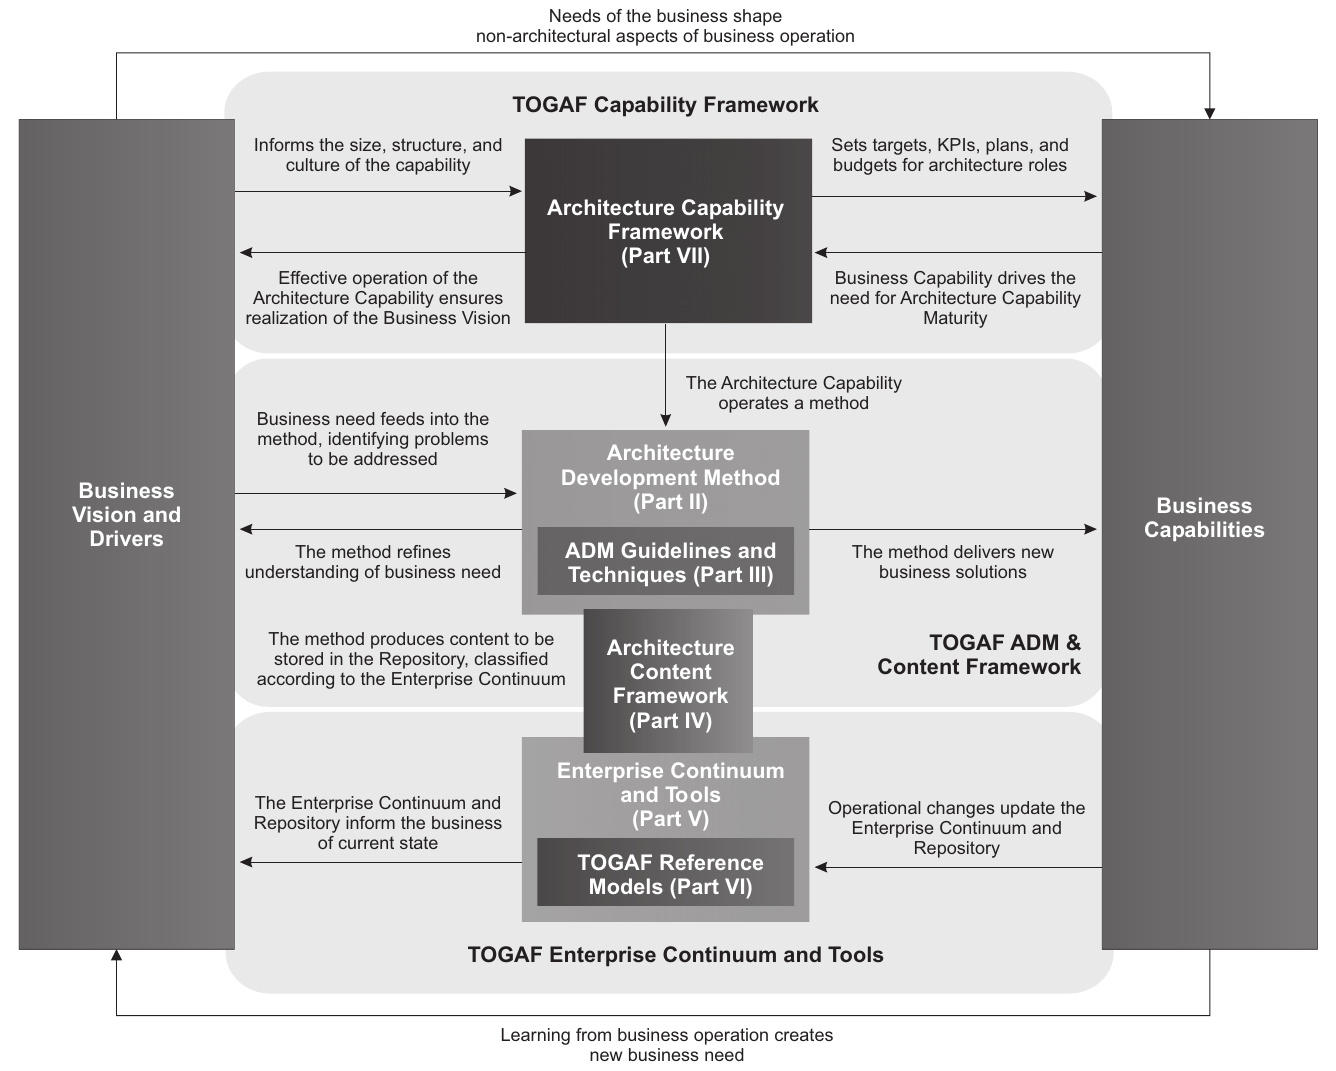
\includegraphics[width=.70\textwidth]{../figures/togaf}
			\end{center}
		\end{frame}
	}
	
	\begin{frame}
		\frametitle{Komponen-komponen TOGAF}
		\begin{itemize}
			\item Business Visions and Drivers
			\item Business Capabilities
			\item Architecture Capability Framework
			\item Architecture Development Method
			\item ADM Guidelines and Techniques
			\item Architecture Governance Frameworks
			\item Architecture Content Framework
			\item Deliverables, Artifacts, and Building Blocks
			\item Enterprise Continuum and Tools
			\item Architecture Repository
			\item TOGAF Reference Models
		\end{itemize}
	\end{frame}
	
	\begin{frame}
		\frametitle{Visi dan Penggerak Bisnis di TOGAF}
		\begin{itemize}
			\item Visi bisnis adalah pandangan tentang tujuan dan masa depan organisasi.
			\item Penggerak bisnis adalah faktor-faktor yang mendorong perubahan dalam organisasi.
			\item TOGAF menggunakan visi dan penggerak bisnis untuk membantu mendefinisikan arsitektur perusahaan.
			\item Visi dan penggerak bisnis dikembangkan selama fase Preliminary dan Architecture Vision dari ADM.
			\item Dalam TOGAF, penggerak bisnis dapat mencakup faktor-faktor seperti perubahan teknologi, perubahan pasar, atau perubahan regulasi.
		\end{itemize}
	\end{frame}
	
	\begin{frame}
		\frametitle{Kemampuan Bisnis di TOGAF}
		\begin{itemize}
			\item Kemampuan bisnis adalah kombinasi dari orang, proses, dan teknologi yang memungkinkan suatu organisasi mencapai tujuannya.
			\item TOGAF memandang kemampuan bisnis sebagai bagian integral dari arsitektur perusahaan.
			\item Pemahaman yang baik tentang kemampuan bisnis dapat membantu dalam merancang dan implementasi arsitektur yang efektif.
			\item Kemampuan bisnis diidentifikasi dan didefinisikan selama proses ADM.
			\item Mereka kemudian digunakan untuk membantu dalam desain dan implementasi arsitektur.
		\end{itemize}
	\end{frame}
	
	{
		\setbeamertemplate{frametitle}{}
		\setbeamertemplate{navigation symbols}{}
		\setbeamertemplate{footline}{}		
		\begin{frame}
			\frametitle{Architecture Capability Framework}
			\begin{center}
				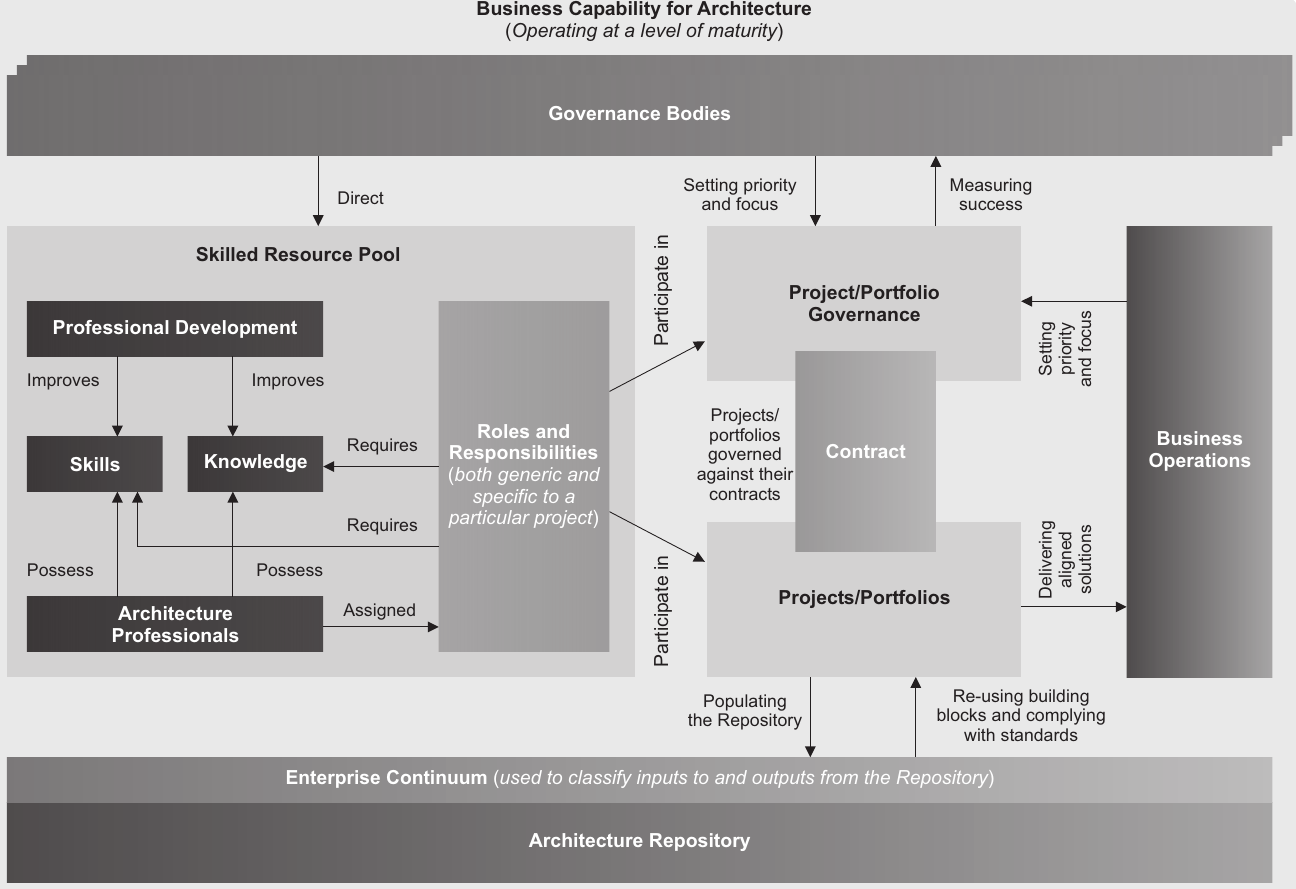
\includegraphics[width=.80\textwidth]{../figures/architecture_capability_framework}
			\end{center}
		\end{frame}
	}
	
	\begin{frame}
		\frametitle{Kerangka Kemampuan Arsitektur TOGAF}
		\begin{itemize}
			\item TOGAF 9 menyediakan Architecture Capability Framework yang merupakan kumpulan dari bahan referensi dan pedoman untuk membangun fungsi arsitektur
			atau kemampuan dalam organisasi.
			\item Terdiri dari tujuh kategori: membangun kemampuan arsitektur, papan arsitektur, kepatuhan arsitektur, kontrak arsitektur, tata kelola arsitektur, model kematangan arsitektur, dan kerangka keterampilan arsitektur.
			\item Setiap kategori mencakup seperangkat kemampuan yang diperlukan untuk menghasilkan arsitektur perusahaan yang efektif.
			\item Menggunakan Kerangka Kemampuan, organisasi dapat mengidentifikasi dan menutupi celah dalam kemampuan mereka.
		\end{itemize}
	\end{frame}
	
	\begin{frame}
		\frametitle{Isi Kerangka Kemampuan Arsitektur TOGAF}
		\begin{itemize}
			\item \textbf{Mendirikan Arsitektur Kemampuan}. Pedoman mendirikan Arsitektur Kemampuan
			dalam sebuah organisasi.
			\item \textbf{Dewan Arsitektur}. Pedoman pendirian dan pengoperasian Dewan Arsitektur perusahaan.
			\item \textbf{Kepatuhan Arsitektur}. Pedoman untuk memastikan kepatuhan proyek Arsitektur.
			\item \textbf{Kontrak Arsitektur}. Pedoman untuk mendefinisikan dan menggunakan Arsitektur Kontrak.
			\item \textbf{Tata Kelola Arsitektur}. Kerangka dan pedoman untuk Arsitektur Pemerintahan.
			\item \textbf{Model Kematangan Arsitektur}. Teknik untuk mengevaluasi dan mengukur suatu kematangan organisasi dalam arsitektur perusahaan.
			\item \textbf{Kerangka Keterampilan Arsitektur}. Serangkaian peran, keterampilan, dan norma pengalaman untuk staf melakukan pekerjaan arsitektur perusahaan.
		\end{itemize}
	\end{frame}
	
	
	\begin{frame}
		\frametitle{Metode Pengembangan Arsitektur (ADM)}
		\begin{itemize}
			\item ADM adalah proses yang direkomendasikan oleh TOGAF untuk mengembangkan arsitektur perusahaan.
			\item Melibatkan serangkaian fase terorganisir yang membantu dalam perancangan, perencanaan, implementasi, dan pengelolaan arsitektur perusahaan.
			\item Fase-fase tersebut termasuk Visi Arsitektur, Desain Bisnis, Desain Informasi, Desain Teknologi, hingga Implementasi.
			\item ADM membantu organisasi mengelola siklus hidup keseluruhan dari arsitektur perusahaan.
			\item ADM juga memberikan pedoman dan teknik untuk setiap fase dari proses pengembangan.
		\end{itemize}
	\end{frame}
	
	{
		\setbeamertemplate{frametitle}{}
		\setbeamertemplate{navigation symbols}{}
		\setbeamertemplate{footline}{}		
		\begin{frame}
			\frametitle{Architecture Development Method}
			\begin{center}
				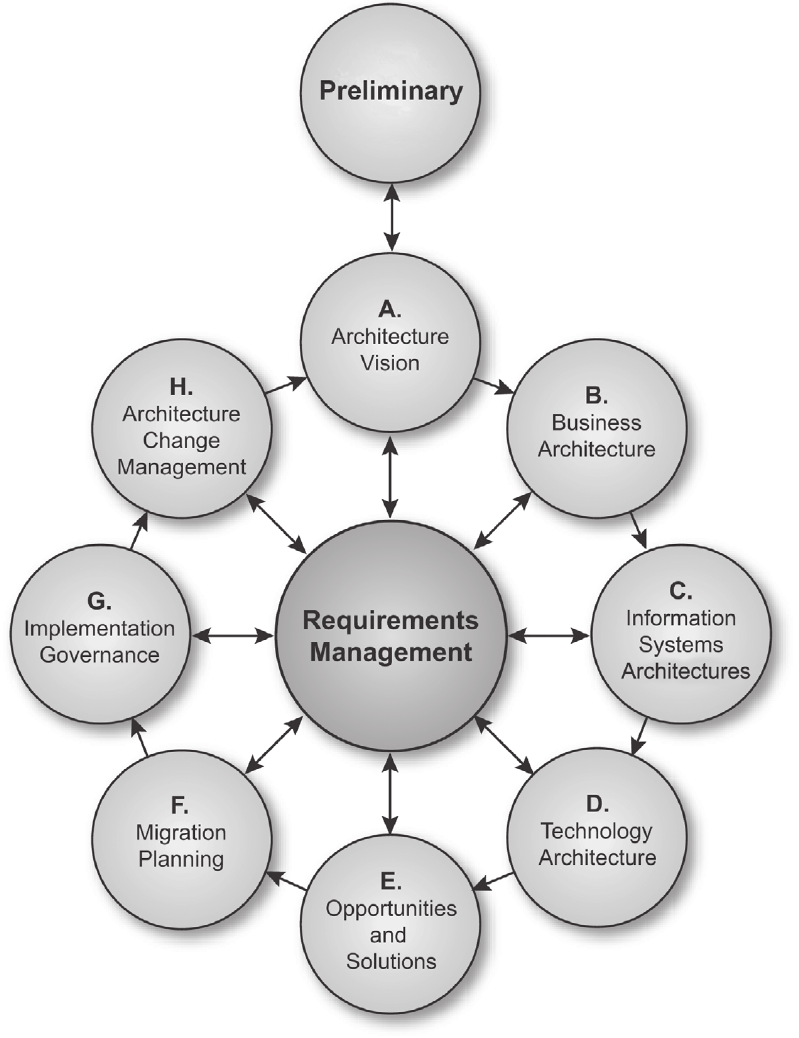
\includegraphics[width=.43\textwidth]{../figures/architecture_development_method}
			\end{center}
		\end{frame}
	}
	
	\begin{frame}
		\frametitle{Pedoman dan Teknik ADM}
		\begin{itemize}
			\item TOGAF menyediakan serangkaian pedoman dan teknik untuk membantu dalam penerapan ADM.
			\item Pedoman ini membantu organisasi dalam menyesuaikan ADM dengan kebutuhan dan konteks mereka sendiri.
			\item Beberapa teknik yang umum digunakan termasuk analisis stakeholder, analisis gap, dan penggunaan matriks arsitektur.
			\item Pedoman dan teknik ini memastikan bahwa proses ADM tetap fokus, efisien, dan efektif.
			\item Mereka juga membantu memastikan bahwa arsitektur yang dihasilkan sesuai dengan tujuan dan sasaran bisnis.
		\end{itemize}
	\end{frame}
	\begin{frame}
		\frametitle{Kerangka Kerja Tata Kelola Arsitektur di TOGAF}
		\begin{itemize}
			\item Tata kelola arsitektur adalah praktik mengelola dan mengendalikan arsitektur perusahaan.
			\item Dalam TOGAF, kerangka kerja tata kelola arsitektur memberikan struktur untuk praktik-praktik ini.
			\item Kerangka kerja ini mencakup aspek seperti struktur organisasi, peran dan tanggung jawab, proses, dan metode komunikasi.
			\item Tata kelola arsitektur juga melibatkan pembuatan dan pemeliharaan artefak seperti prinsip arsitektur, model arsitektur, dan roadmap arsitektur.
			\item Tujuan utamanya adalah untuk memastikan bahwa semua proyek tetap selaras dengan arsitektur perusahaan dan strategi bisnis secara keseluruhan.
		\end{itemize}
	\end{frame}
	
	\begin{frame}
		\frametitle{Kerangka Konten Arsitektur}
		\begin{itemize}
			\item Kerangka Konten Arsitektur mendefinisikan jenis konten arsitektural yang diperlukan untuk mencakup keseluruhan domain bisnis.
			\item Ini memandu proses identifikasi, organisasi, dan pengembangan artefak.
			\item Kerangka Konten Arsitektur terdiri dari tiga komponen utama: Deliverables, Artefak, dan Building Blocks.
			\item Deliverables adalah hasil kerja yang diberikan kepada pemangku kepentingan. Artefak adalah bagian dari Deliverables yang mendeskripsikan arsitektur.
			\item Building Blocks adalah komponen fisik, logis, atau konseptual dari sistem bisnis atau IT.
		\end{itemize}
	\end{frame}
	
	
	
	\begin{frame}
		\frametitle{Deliverables, Artefak, dan Building Blocks di TOGAF}
		\begin{itemize}
			\item Deliverables adalah hasil kerja arsitektur yang diberikan kepada pemangku kepentingan.
			\item Artefak adalah bagian dari Deliverables yang mendeskripsikan arsitektur dalam berbagai tingkat detail.
			\item Building Blocks adalah komponen fisik, logis, atau konseptual dari sistem bisnis atau IT.
			\item Contoh Deliverables: Dokumen Visi Arsitektur, Rencana Migrasi.
			\item Contoh Artefak: Diagram Data, Diagram Aplikasi. Contoh Building Blocks: server, aplikasi, database.
		\end{itemize}
	\end{frame}
	
	{
		\setbeamertemplate{frametitle}{}
		\setbeamertemplate{navigation symbols}{}
		\setbeamertemplate{footline}{}		
		\begin{frame}
			\frametitle{Architecture Deliverables}
			\begin{center}
				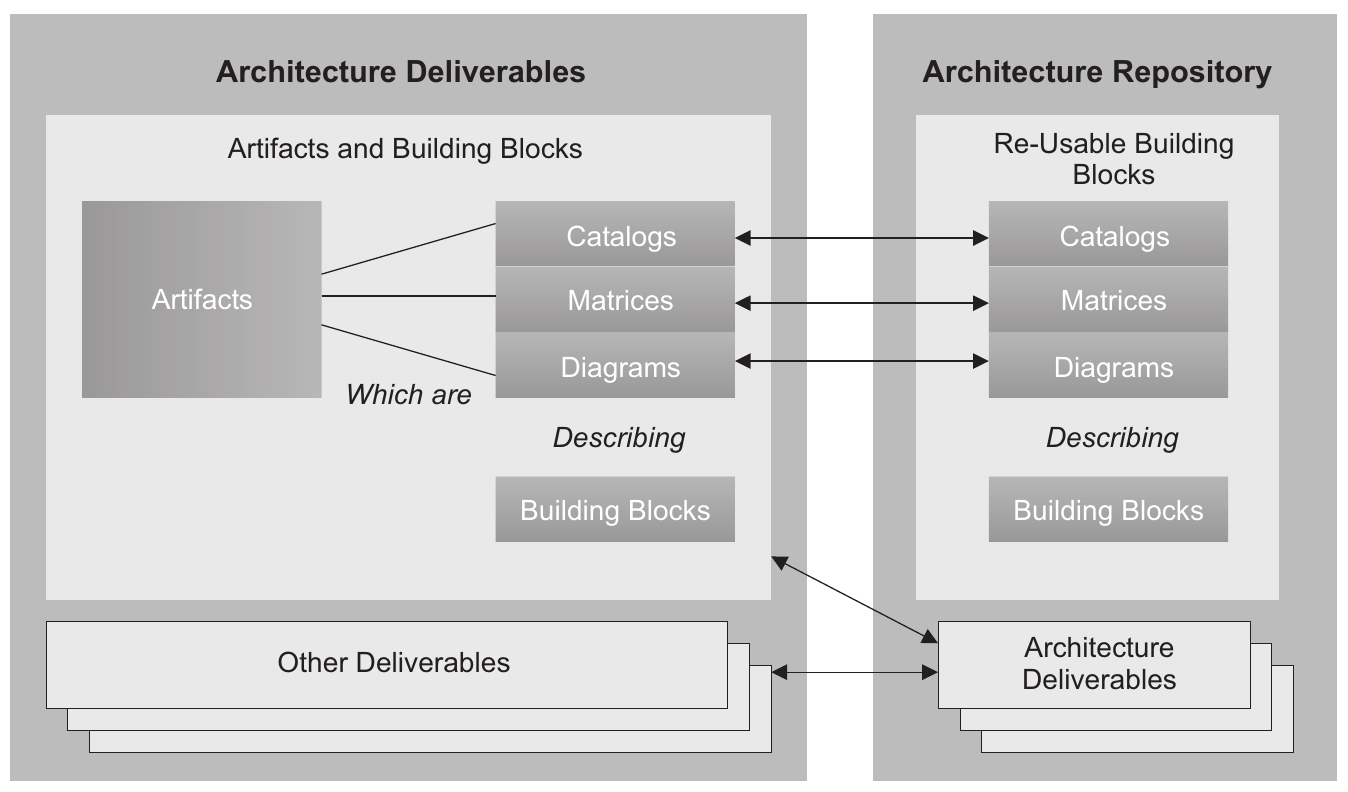
\includegraphics[width=.95\textwidth]{../figures/architecture_deliverables}
			\end{center}
		\end{frame}
	}
	
	
	
	\begin{frame}
		\frametitle{Kontinum dan Alat Perusahaan}
		\begin{itemize}
			\item Kontinum Perusahaan adalah pandangan "virtual" atau panduan yang menyediakan konteks untuk memahami dan mengelola artefak arsitektur.
			\item Ini membantu organisasi mengidentifikasi dan memanfaatkan artefak yang relevan berdasarkan kebutuhan mereka.
			\item Alat Perusahaan adalah alat dan teknik yang digunakan untuk mendukung pembuatan, manajemen, dan penggunaan arsitektur.
			\item Contoh alat ini termasuk perangkat lunak pemodelan, alat manajemen proyek, dan alat dokumentasi.
			\item Alat ini mendukung organisasi dalam menerapkan dan mengelola arsitektur perusahaan mereka.
		\end{itemize}
	\end{frame}
	
	{
		\setbeamertemplate{frametitle}{}
		\setbeamertemplate{navigation symbols}{}
		\setbeamertemplate{footline}{}		
		\begin{frame}
			\frametitle{Architecture Continuum}
			\begin{center}
				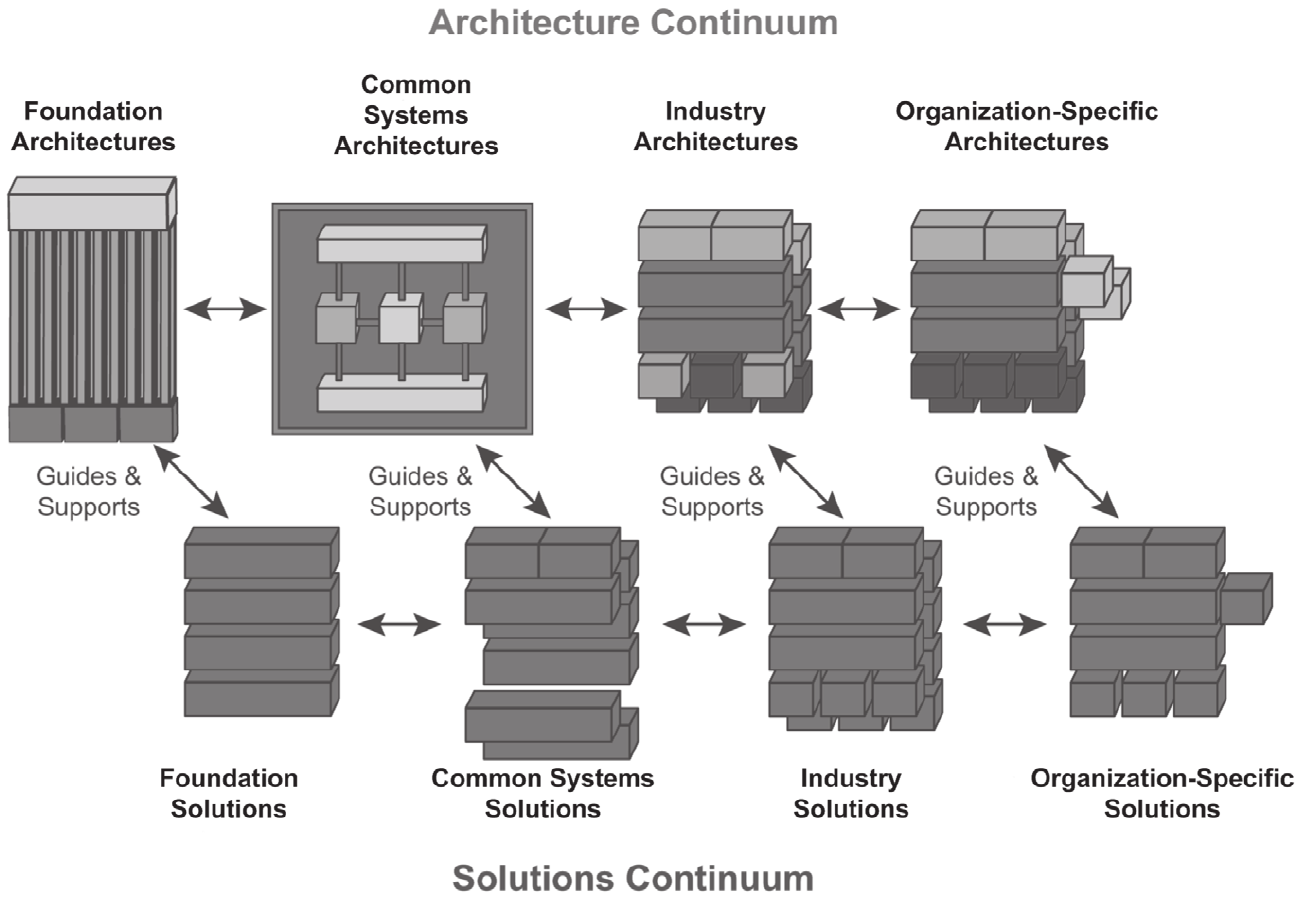
\includegraphics[width=.80\textwidth]{../figures/enterprise_continuum}
			\end{center}
		\end{frame}
	}
	
	\begin{frame}
		\frametitle{Repositori Arsitektur di TOGAF}
		\begin{itemize}
			\item Repositori Arsitektur adalah tempat penyimpanan yang terorganisir untuk semua artefak yang dihasilkan oleh arsitek selama siklus hidup ADM.
			\item Repositori ini membantu dalam penyimpanan, pengelolaan, dan penggunaan kembali informasi arsitektural.
			\item Repositori ini melibatkan tiga level: Foundation Architecture, Common Systems Architecture, dan Industry Architecture.
			\item Repositori ini juga mendukung pengelolaan dan pemantauan Kontrak Arsitektur.
			\item Repositori ini memudahkan manajemen artefak dan deliverable dalam lingkungan multi-proyek.
		\end{itemize}
	\end{frame}
	
	
	{
		\setbeamertemplate{frametitle}{}
		\setbeamertemplate{navigation symbols}{}
		\setbeamertemplate{footline}{}		
		\begin{frame}
			\frametitle{Architecture Repository}
			\begin{center}
				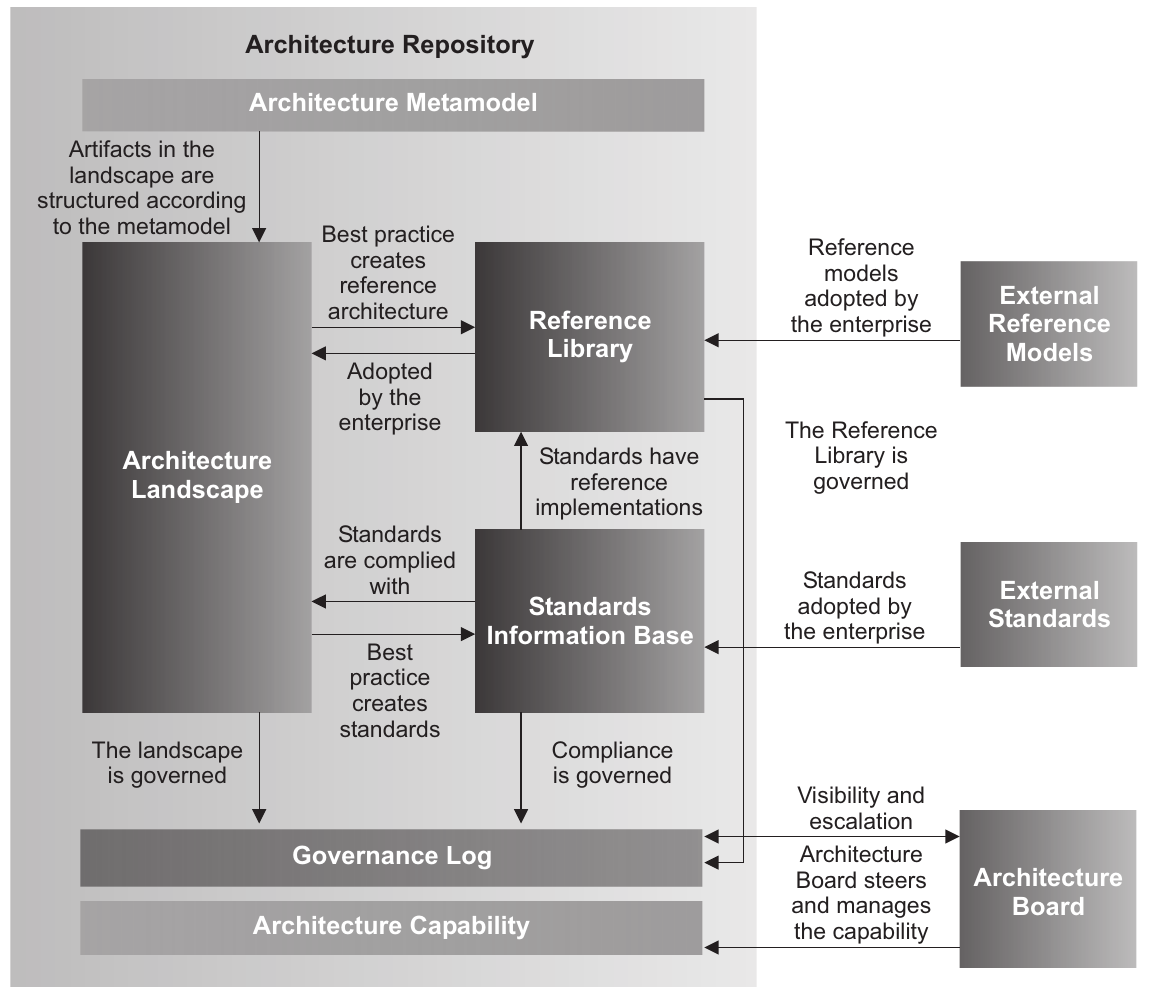
\includegraphics[width=.65\textwidth]{../figures/architecture_repository}
			\end{center}
		\end{frame}
	}
	
	
	
	
	\begin{frame}
		\frametitle{Model Referensi TOGAF}
		\begin{itemize}
			\item Model Referensi TOGAF adalah kerangka kerja yang memberikan titik awal yang bermanfaat untuk organisasi yang mencari bantuan dengan inisiatif arsitektur mereka.
			\item Ini memberikan model dasar yang dapat digunakan sebagai dasar untuk mengembangkan arsitektur yang lebih spesifik dan rinci.
			\item Model Referensi TOGAF meliputi Model Referensi Arsitektur Teknis (TRM) dan Model Referensi Integrasi Sistem Terbuka (III-RM).
			\item TRM memberikan model dan taksonomi umum untuk teknologi yang mendukung bisnis aplikasi, seperti sistem operasi, perangkat keras, dan jaringan.
			\item III-RM memberikan model untuk arsitektur dan komponen yang memungkinkan portabilitas, interoperabilitas, dan reuse aplikasi yang lebih besar.
		\end{itemize}
	\end{frame}
	
	{
		\setbeamertemplate{frametitle}{}
		\setbeamertemplate{navigation symbols}{}
		\setbeamertemplate{footline}{}		
		\begin{frame}
			\frametitle{Technical Reference Model}
			\begin{center}
				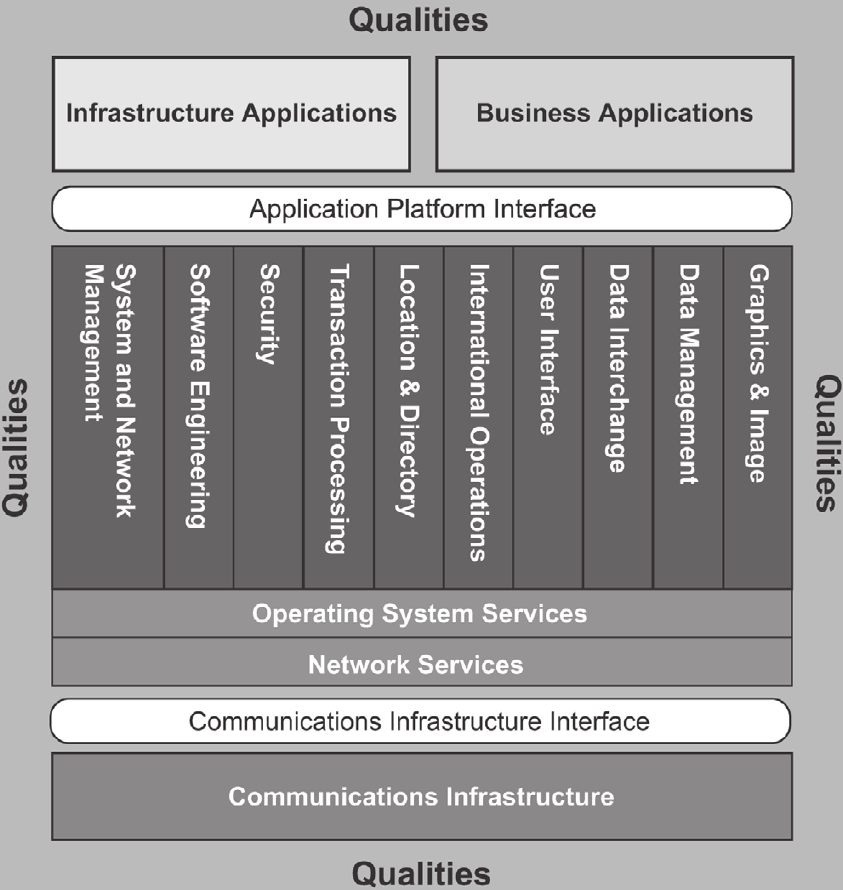
\includegraphics[width=.53\textwidth]{../figures/detailed_technical_reference_model}
			\end{center}
		\end{frame}
	}
	
	{
		\setbeamertemplate{frametitle}{}
		\setbeamertemplate{navigation symbols}{}
		\setbeamertemplate{footline}{}		
		\begin{frame}
			\frametitle{Integrated Information Infrastructure Reference Model}
			\begin{center}
				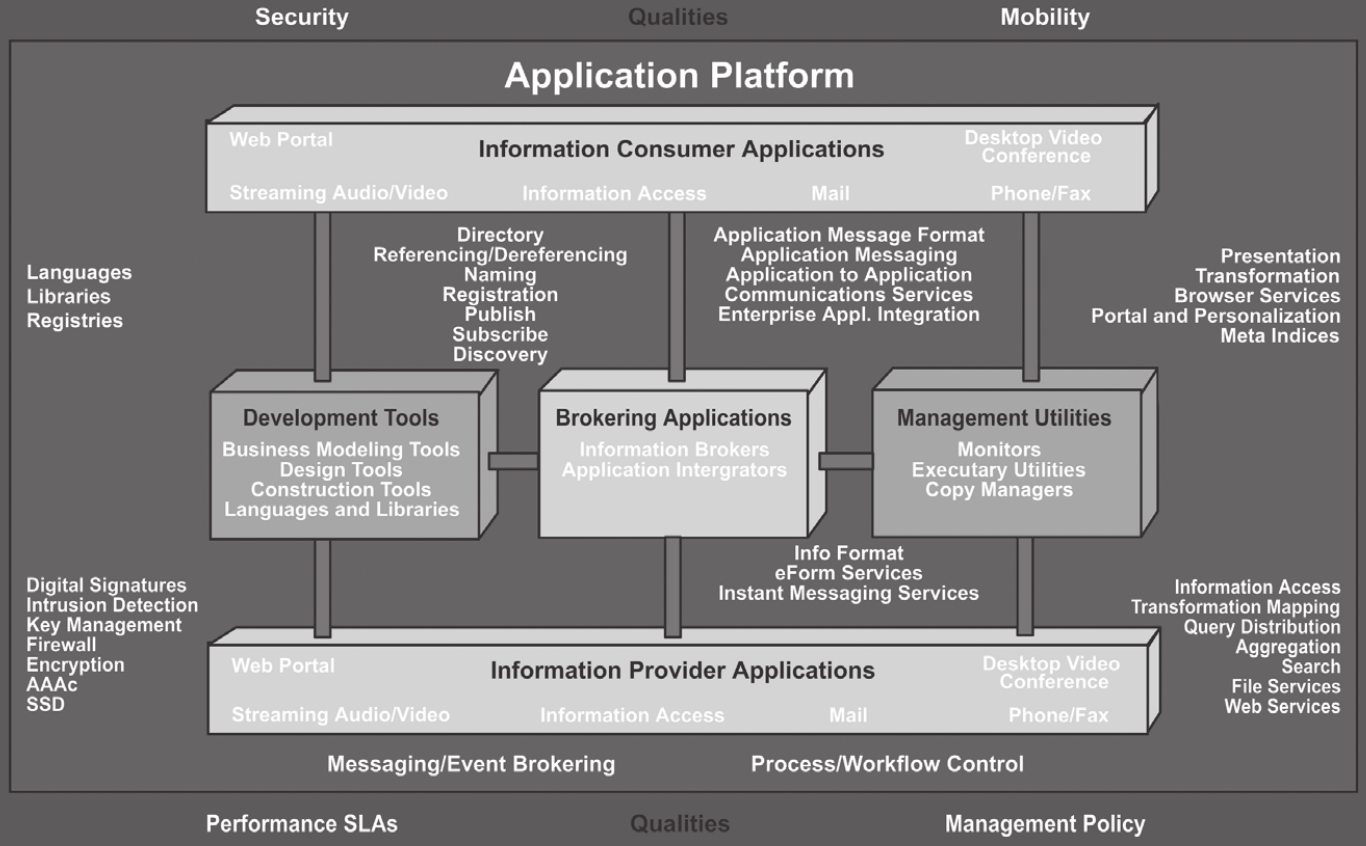
\includegraphics[width=.90\textwidth]{../figures/integrated_information_infrastructure_reference_model}
			\end{center}
		\end{frame}
	}
	
	\begin{frame}
		\frametitle{Ringkasan}
		\begin{itemize}
			\item TOGAF adalah kerangka kerja arsitektur perusahaan yang komprehensif yang membantu organisasi dalam merancang, merencanakan, menerapkan, dan mengelola arsitektur informasi mereka.
			\item TOGAF melibatkan berbagai aspek seperti visi dan driver bisnis, kapabilitas bisnis, kerangka kerja kapabilitas, metode pengembangan arsitektur, dan lainnya.
			\item Dalam TOGAF, artefak, deliverable, dan building blocks digunakan untuk membantu dalam proses pengembangan arsitektur.
			\item Kontinum dan alat perusahaan di TOGAF membantu organisasi memahami dan memanfaatkan kerangka kerja ini secara efektif.
			\item Repositori Arsitektur dan Model Referensi TOGAF adalah komponen acuan pengetahuan yang penting untuk mendukung proses ADM.
		\end{itemize}
	\end{frame}
	
\end{document}
